\documentclass{article}

% Language setting
% Replace `english' with e.g. `spanish' to change the document language
\usepackage[danish]{babel}
% Set page size and margins
% Replace `letterpaper' with `a4paper' for UK/EU standard size
\usepackage[a4paper,top=2cm,bottom=2cm,left=3cm,right=3cm,marginparwidth=1.75cm]{geometry}

% Useful packages
\usepackage{amsmath}
\usepackage{graphicx}
\usepackage[colorlinks=true, allcolors=blue]{hyperref}
\usepackage{array}
\usepackage{subfig}
\usepackage{subfigure}
\usepackage{titlesec}

\title{CDIO delopgave 0}
\author{Jakob Agergaard}


\begin{document}

\titlespacing{\section}
    {0pt}{2em}{1em}




\begin{titlepage}
\begin{center}

    
\includegraphics[width=0.25\textwidth]{Billeder/DTULogo.png} \\
    \vspace{0.5cm}
    \Large
    \textbf{02314\hspace{1cm}62531\hspace{1cm}62532} \\
    Indledende programmering, Udviklingsmetoder til IT-systemer og Versionsstyring og testmetoder
    \vspace{0.4cm}
    \hrule
    
    \vspace*{0.5cm}
    \huge
    \textbf{CDIO delopgave 0}\\
    \LARGE
    Gruppe 17
    \vspace{0.5cm}
    \hrule
    \vspace{0.2cm}

    \large
    \begin{tabular}{m{10em} m{8em} m{8em} m{10em}}
    Jakob Skov Agergaard\vfill s224570 & 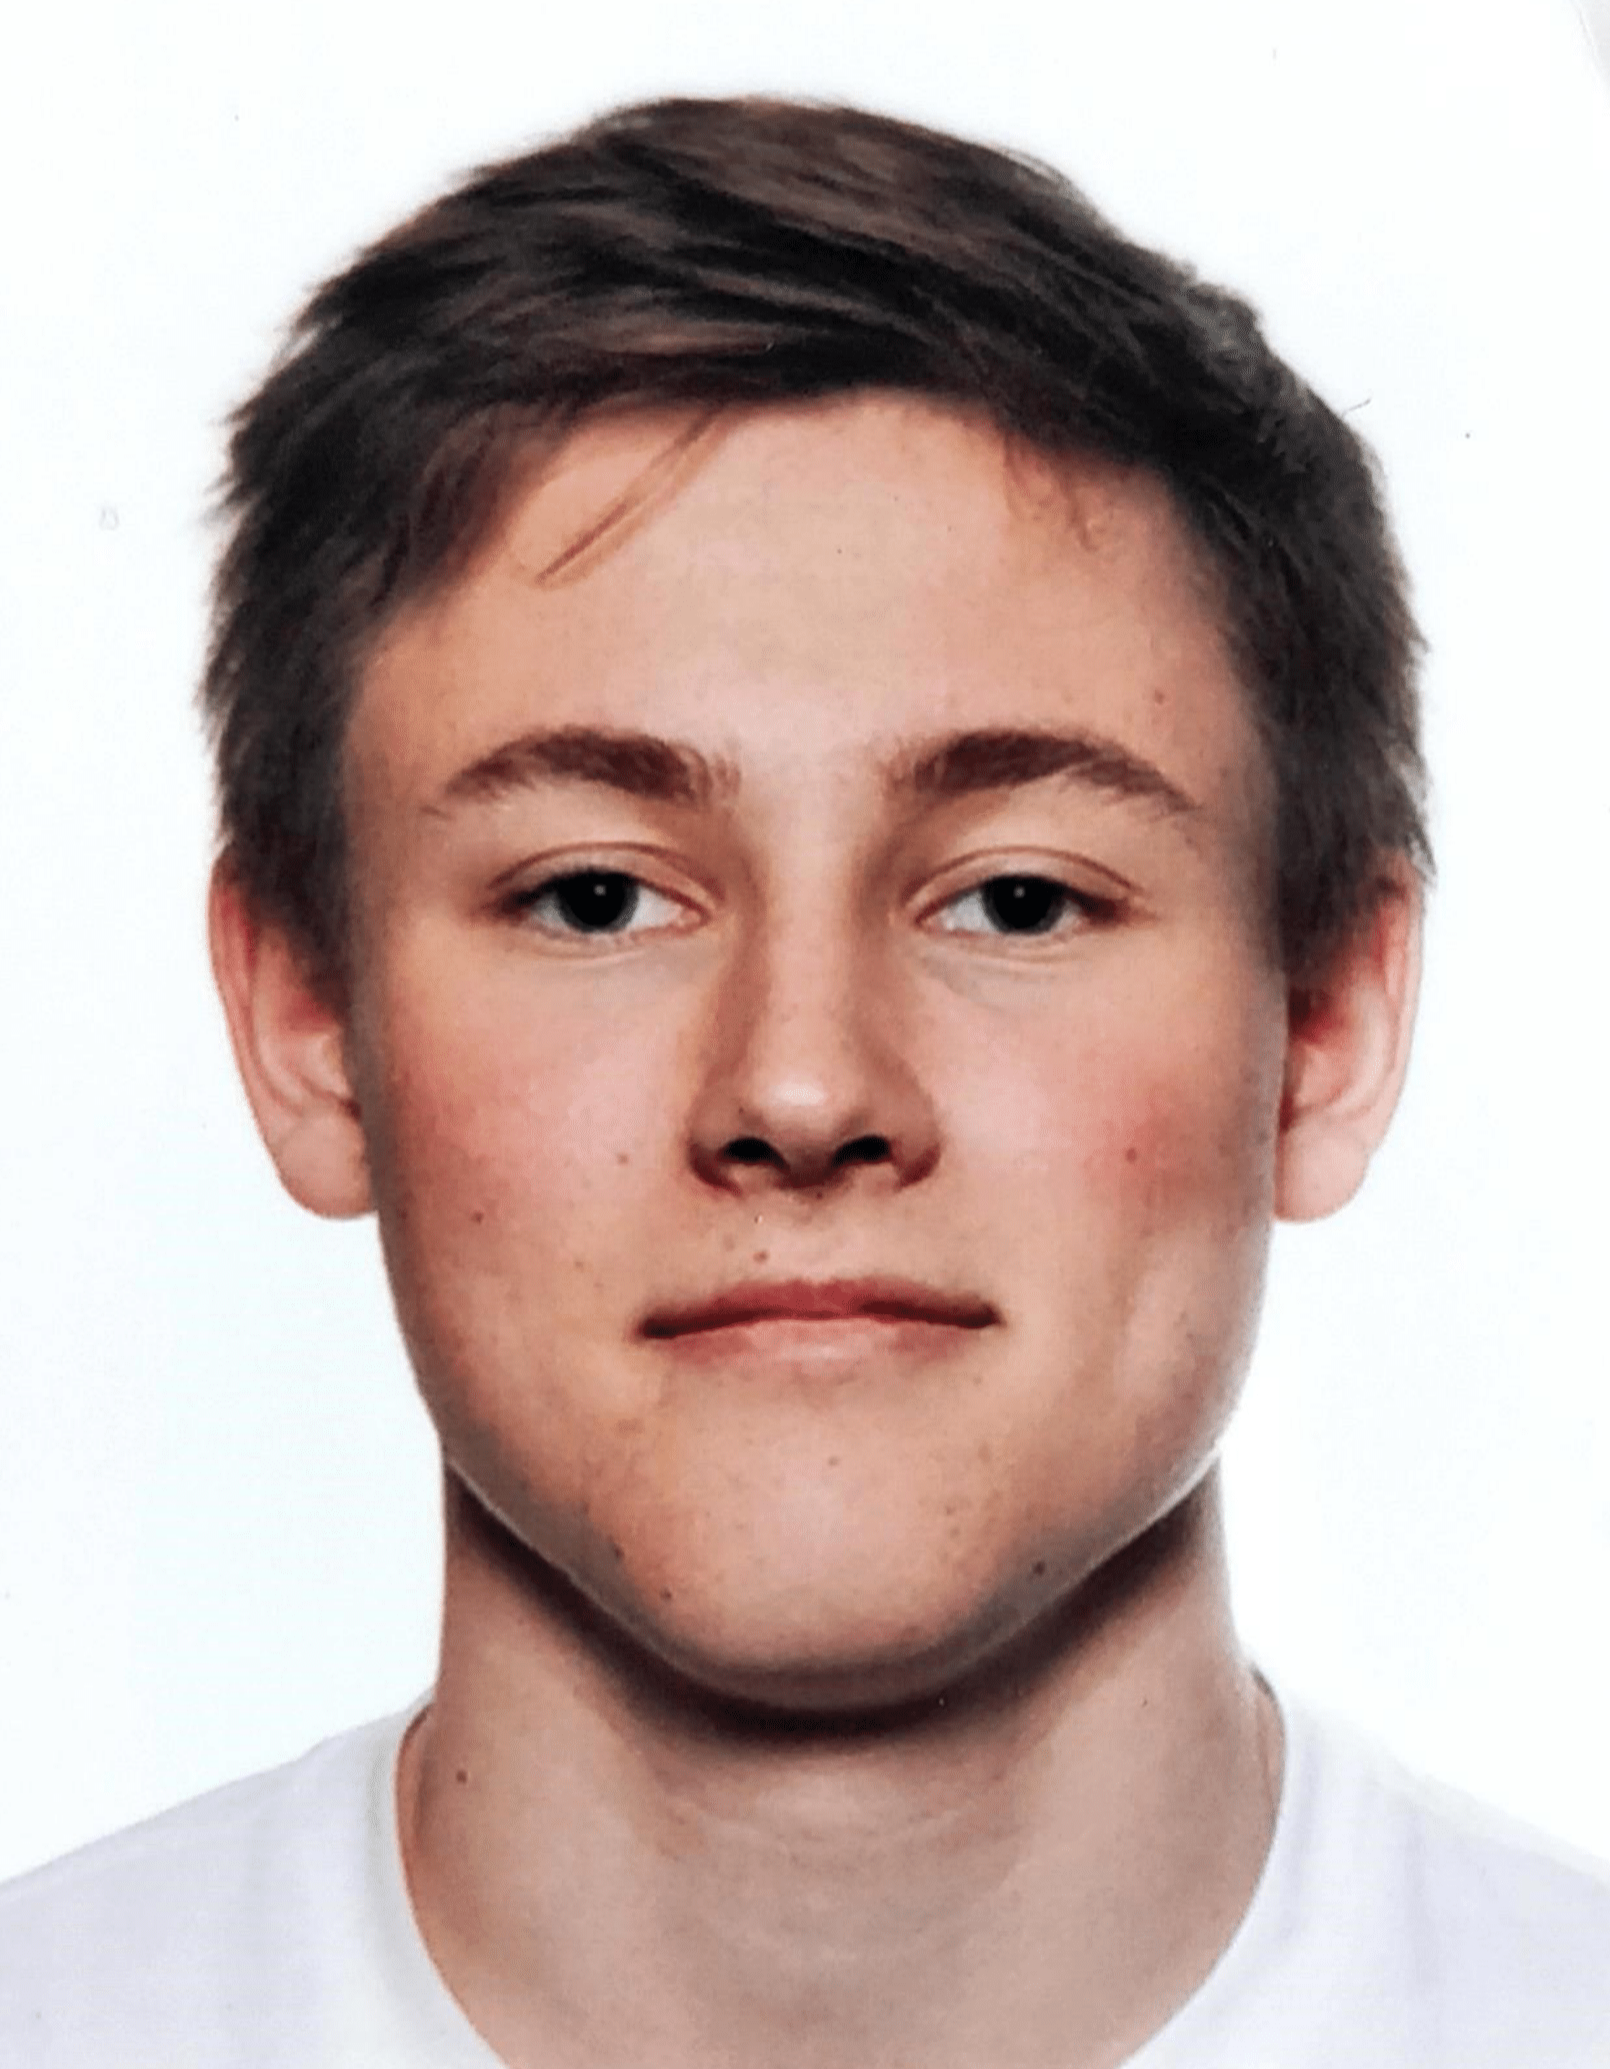
\includegraphics[width=0.2\textwidth]{Billeder/JakobFoto.png} & 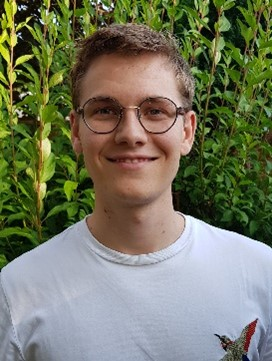
\includegraphics[width=0.2\textwidth]{Billeder/PhilipFoto.jpg} & Philip Muff Førrisdahl\vfill s224566 \\
    Mads Fogelberg Hansen\vfill s224563 & 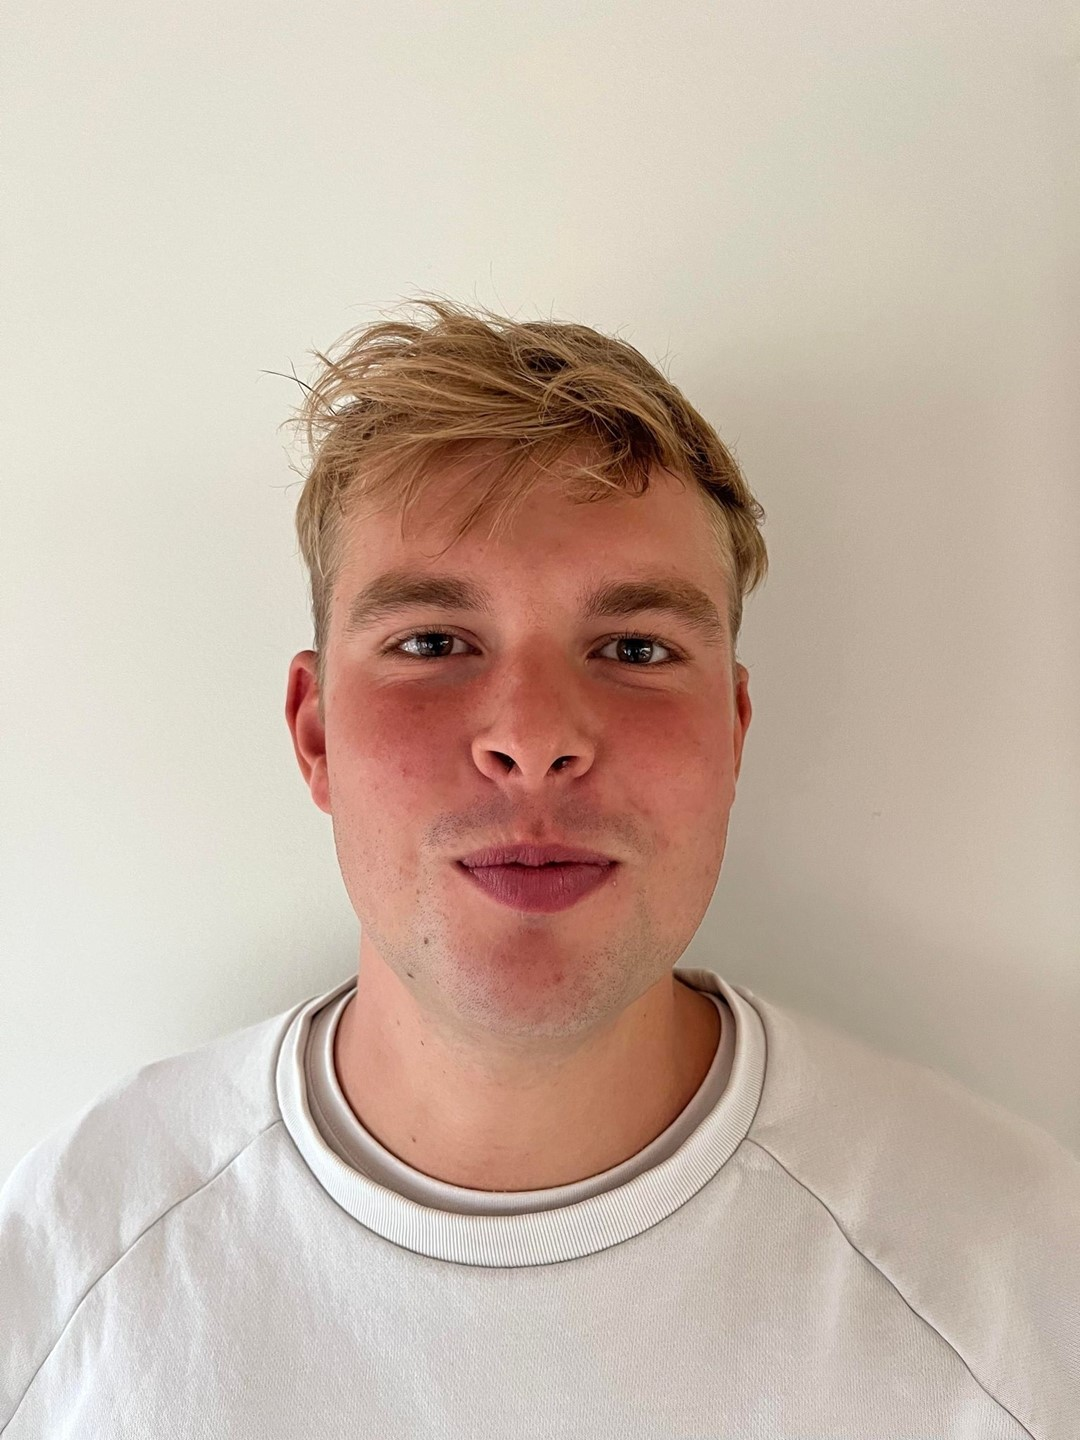
\includegraphics[width=0.2\textwidth]{Billeder/FotoMads.jpg} & 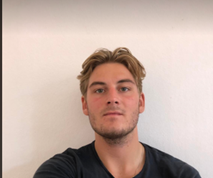
\includegraphics[width=0.2\textwidth]{Billeder/EsbenFoto.png} & Esben Skovmand Elnegaard \vfill s224555  \\
    Jarl Boyd Roest\vfill s224556 & 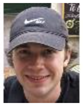
\includegraphics[width=0.2\textwidth]{Billeder/JarlFoto.png}
    \end{tabular}

    \vfill
    
    
    \vspace{1cm}
    \LARGE
    18. september 2022

    \vspace{1cm}
    
\end{center}
\end{titlepage}


\normalsize
\begin{abstract}
     Her kommer der et resume af opgaven
\end{abstract}

\tableofcontents

\section{Timeregnskab}

\section{Indledning}

Her kommer indledningen...

\section{Projekt-planlægning}

\section{Krav/Analyse}

\section{Design}

\section{Implementering}

\section{Test}

\section{Konklusion}

\section{Bilag}
\subsection{Litteratur}
\subsection{Kode}

\end{document}